CSCS is deploying isolated clusters (vClusters) on the \crayex system Alps, to provide services to a wider range of user domains, each with their own software, security, reliability and scaling requirements.
The vClusters can be customized for the target use cases, as an alternative to providing one large system with a ``one size fits all'' programming environment, storage and job scheduler configuration.

CSCS aims to reduce the complexity of the software installed on each cluster by providing use case-specific user environments on vClusters; specifically by providing the smallest possible set of compilers, libraries and tools optimized for each use case's requirements, node architecture and the Slingshot 11 interconnect.
An obvious use case for the environments is single purpose clusters, for example for the weather service's production cluster.
Alternatively, the multiple use-case specific environments can be provided on general-purpose HPC clusters, and loaded according to the user's needs.

This is at odds with the widely-adopted approach to providing software on \crayex systems, namely installing the Cray Programming Environment (CPE), and building use-case specific software not provided by CPE on a shared file system, as illustrated in~\fig{fig:stacks}(a).
To date CSCS has provided such a one-size-fits-all environment, similarly to other HPC sites, using the EasyBuild to to provide additional software built and maintained by CSCS~\cite{forai:cug16}.


\begin{figure*}[htp!]
    \begin{center}
        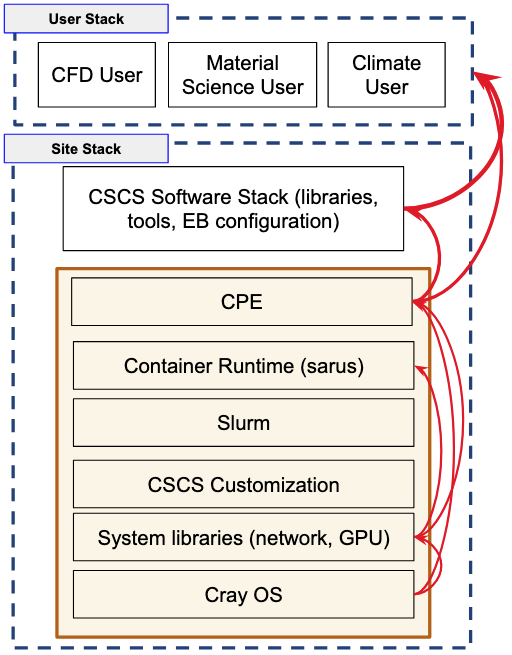
\includegraphics[width=0.35\textwidth]{./images/stack-old.png}
        \hspace{2.5cm}
        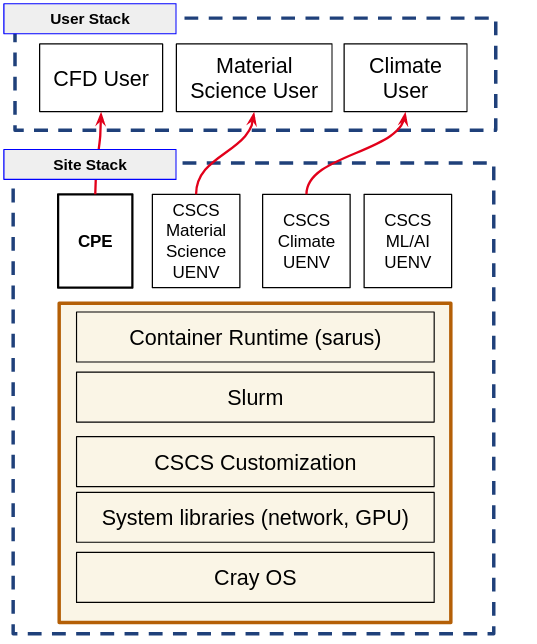
\includegraphics[width=0.35\textwidth]{./images/stack-new.png}
        \\
        \textbf{(a)} \hspace{9cm} \textbf{(b)}\\
    \end{center}
    \caption{
        \textbf{(a)}:
        The "standard" HPE-EX software stack, with the Cray OS, drivers, CPE and some site software in the system image, site-provided software installed on a shared file system, and software installed by users that depends can depend on different software layers underneath.
        The red arrows indicate where changes on one layer, can have a knock on effect on other software layers, requireing rebuilds or reconfiguration when they are changed.\\
        \textbf{(b)}:
        The Alps software stack, with the programming environment moved out of the base image.
        Multiple programming environments can be deployed on top of this architecture, including the CPE and alternative PEs discussed in~\sect{sec:spack-stacks} that are mounted at runtime in a new mount namespace by users.
    }
    \label{fig:stacks}
\end{figure*}

The CPE provides a very wide range of software -- including compilers, scientific libraries, communication libraries, debuggers and profiling tools -- all optimised for the node and network architecture of the system.
The CPE continues to evolve and expand in response to changing requirements, for example adding software packages for ML/AI, with quarterly releases to address bugs, improve performance and add features.
As such, while CPE a good general purpose environment for users, using it as a layer in HPC software stacks it is at odds with our aim of reducing the complexity of stacks.
\begin{itemize}
    \item No single use-case or domain will use more than a small subset of the features provided by the CPE;
    \item The CPE released on a quarterly cycle, so the lead time between identifying an issue and a fix available and tested on site can be expected to be in the order of 3-6 months;
\end{itemize}
By striking a balance between long term stability and providing up-to date software versions, it can't satisfy use cases that require either.

The work presented in this paper utilizes \spack and SquashFS images to build and deploy software stacks on top of a simplified base image that provides only the neccessarily vendor-specific libraries, e.g. libfabric, see~\fig{fig:stacks}.
Such a base image is updated less frequently than CPE, so the frequency of rebuilds will be lower than if we built our stack on top of CPE, and the number of system dependencies that could require intervention are fewer.

The result is compact, testable, reproducable and optimized software environments based on a descriptive recipe that can be updated independently of the CPE release cycle.

%\begin{enumerate}
%    \item long term stability -- software stack configuration can be maintained for longer
%    \begin{itemize}
%        \item requirement: reproducable builds
%        \item requirement: concise descriptive  recipes
%        \item requirement: minimise system requirements to only the bare minimum (no CPE)
%    \end{itemize}
%    \item rolling releases and fast fixes -- be able to rebuild and reconfigure at any point
%    \item provide use-case or application specific environments (only provide the required minimum)
%    \begin{itemize}
%        \item requirement: versioning of environments
%        \item requirement: fast deployment
%    \end{itemize}
%    \item deliver a satisfying user experience
%    \begin{itemize}
%        \item building and configuring software is fast and consistent (not dependent on file system performance).
%        \item compatibility with module, spack, python venv workflows.
%    \end{itemize}
%\end{enumerate}


%%% Local Variables:
%%% TeX-master: "paper"
%%% End:
